%%%%%%%%%%%%%%%%%%%%%%%%%%%%%%%%%%%%%%%%%%%%%%%%%%%%%%%%%%%%%%%%%%%%%%%%%%%%%%%%
\section{About Snakemake}
{   
	\usebackgroundtemplate{
		\vbox to \paperheight{\vfil\hbox to \paperwidth{\hfil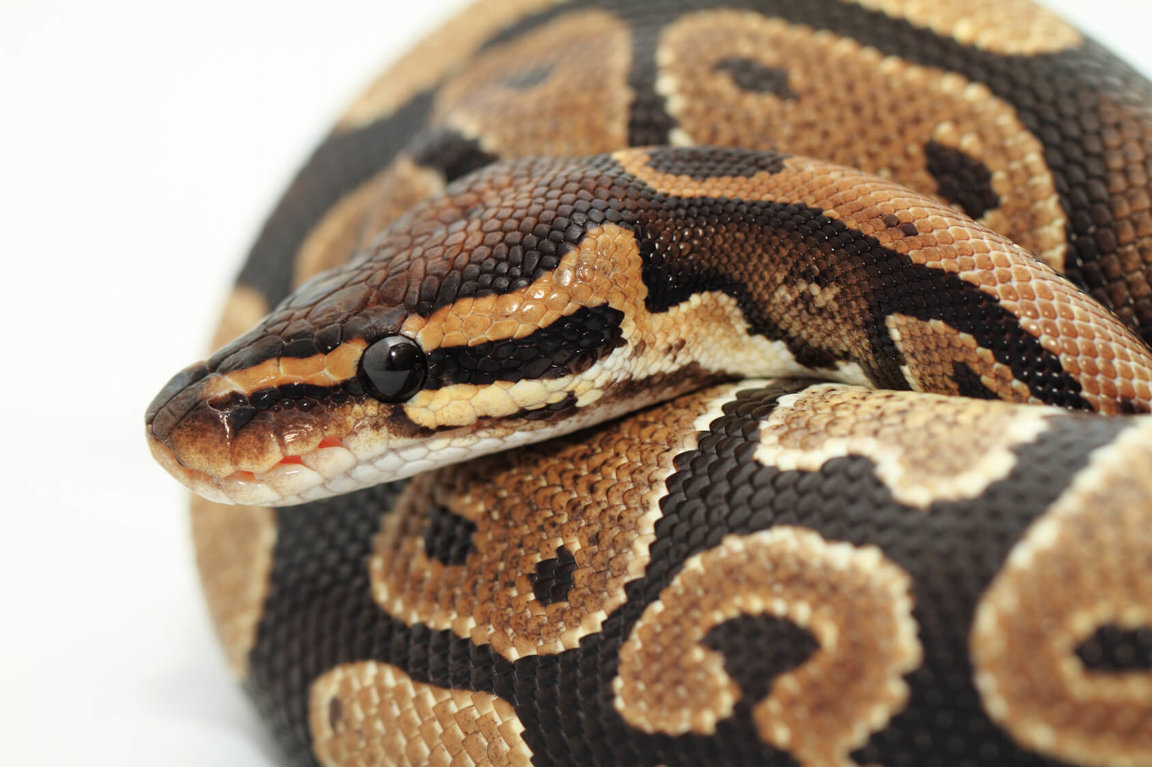
\includegraphics[height=\paperheight]{logos/Wild_Python.jpg}\hfil}\vfil}
	}
	\frame{
		\frametitle{Snakemake}
		\begin{mdframed}[tikzsetting={draw=white,fill=white,fill opacity=0.8,
				line width=0pt},backgroundcolor=none,leftmargin=0,
			rightmargin=150,innertopmargin=4pt,roundcorner=10pt]
			\tableofcontents[currentsection,sections={1-4},hideothersubsections]
		\end{mdframed}
	}
}

%%%%%%%%%%%%%%%%%%%%%%%%%%%%%%%%%%%%%%%%%%%%%%%%%%%%%%%%%%%%%%%%%%%%%%%%%%%%%%%%
\begin{frame}
	\frametitle{What is this about?}
	\begin{question}[Questions]
		\begin{itemize}
			\item What is \Snakemake?
			\item How does it work on a Cluster?
			\item What about other Workflow Management Systems?
		\end{itemize}
	\end{question}
	\begin{docs}[Objectives]
		\begin{enumerate}
			\item Introduction to \Snakemake Usage (in-depth introduction for users, only)
			\item Get an Mini-Overview about Workflow Systems
		\end{enumerate}
	\end{docs}
\end{frame}

\subsection{\Snakemake and the Workflow Catalogue}

%%%%%%%%%%%%%%%%%%%%%%%%%%%%%%%%%%%%%%%%%%%%%%%%%%%%%%%%%%%%%%%%%%%%%%%%%%%%%%%%
\begin{frame}
	\frametitle{\Snakemake}
	\begin{figure}
		\centering
		\caption*{\textbf{>1e6} downloads since 2015\newline
			\textbf{>1300} citations\newline
			\textbf{>7} citations per week since 2021}
		
\includegraphics[width=0.6\textwidth]{Snakemake/paper_wall.png}
	\end{figure}
\end{frame}

%%%%%%%%%%%%%%%%%%%%%%%%%%%%%%%%%%%%%%%%%%%%%%%%%%%%%%%%%%%%%%%%%%%%%%%%%%%%%%%%
\begin{frame}
	\frametitle{\Snakemake -- Bioinformatics to Physics}
	Although developed first for Bioinformatics users, meanwhile used 
	\begin{figure}[ht]
		\begin{minipage}[b]{0.45\linewidth}
			\centering
			\vspace{-1em}
			
\includegraphics[width=\textwidth]{logos/bioinformatics.png}
			\vspace{0.5em}
			\caption*{bioformatics, incl. pharmaceutical research, structural biology, etc.}
			\label{fig:a}
		\end{minipage}
		\hspace{0.5cm}
		\begin{minipage}[b]{0.45\linewidth}
			\centering
			\vspace{-0.8em}
			
\includegraphics[width=\textwidth]{logos/physics.png}
			\vspace{0.5em}
			\caption*{experimental physics, fluid dynamics, high energy physics (CERN)}
			\label{fig:b}
		\end{minipage}
	\end{figure}
	%<a href="https://www.flaticon.com/free-icons/bioinformatics" title="bioinformatics icons">Bioinformatics icons created by Freepik - Flaticon</a>
\end{frame}


%%%%%%%%%%%%%%%%%%%%%%%%%%%%%%%%%%%%%%%%%%%%%%%%%%%%%%%%%%%%%%%%%%%%%%%%%%%%%%%%
\begin{frame}
	\frametitle{The \Snakemake{} Catalogue}
	\begin{columns}
		\begin{column}{0.5\textwidth}
			\begin{itemize}[<+->]
				\item Extremely feature rich: \lhref{https://snakemake.github.io/snakemake-workflow-catalog/}{over 1800 workflows (mostly bioinformatics)}
				\item Almost a hundred standardized workflows ready to use (meaning: well documented and with automatic deployment)
				\item Cluster batch systems are supported (and support for various cloud systems, too)
				\item There is an option to include Nextflow wrappers, too.
			\end{itemize}
		\end{column}
		\begin{column}{0.5\textwidth}
			\begin{figure}
				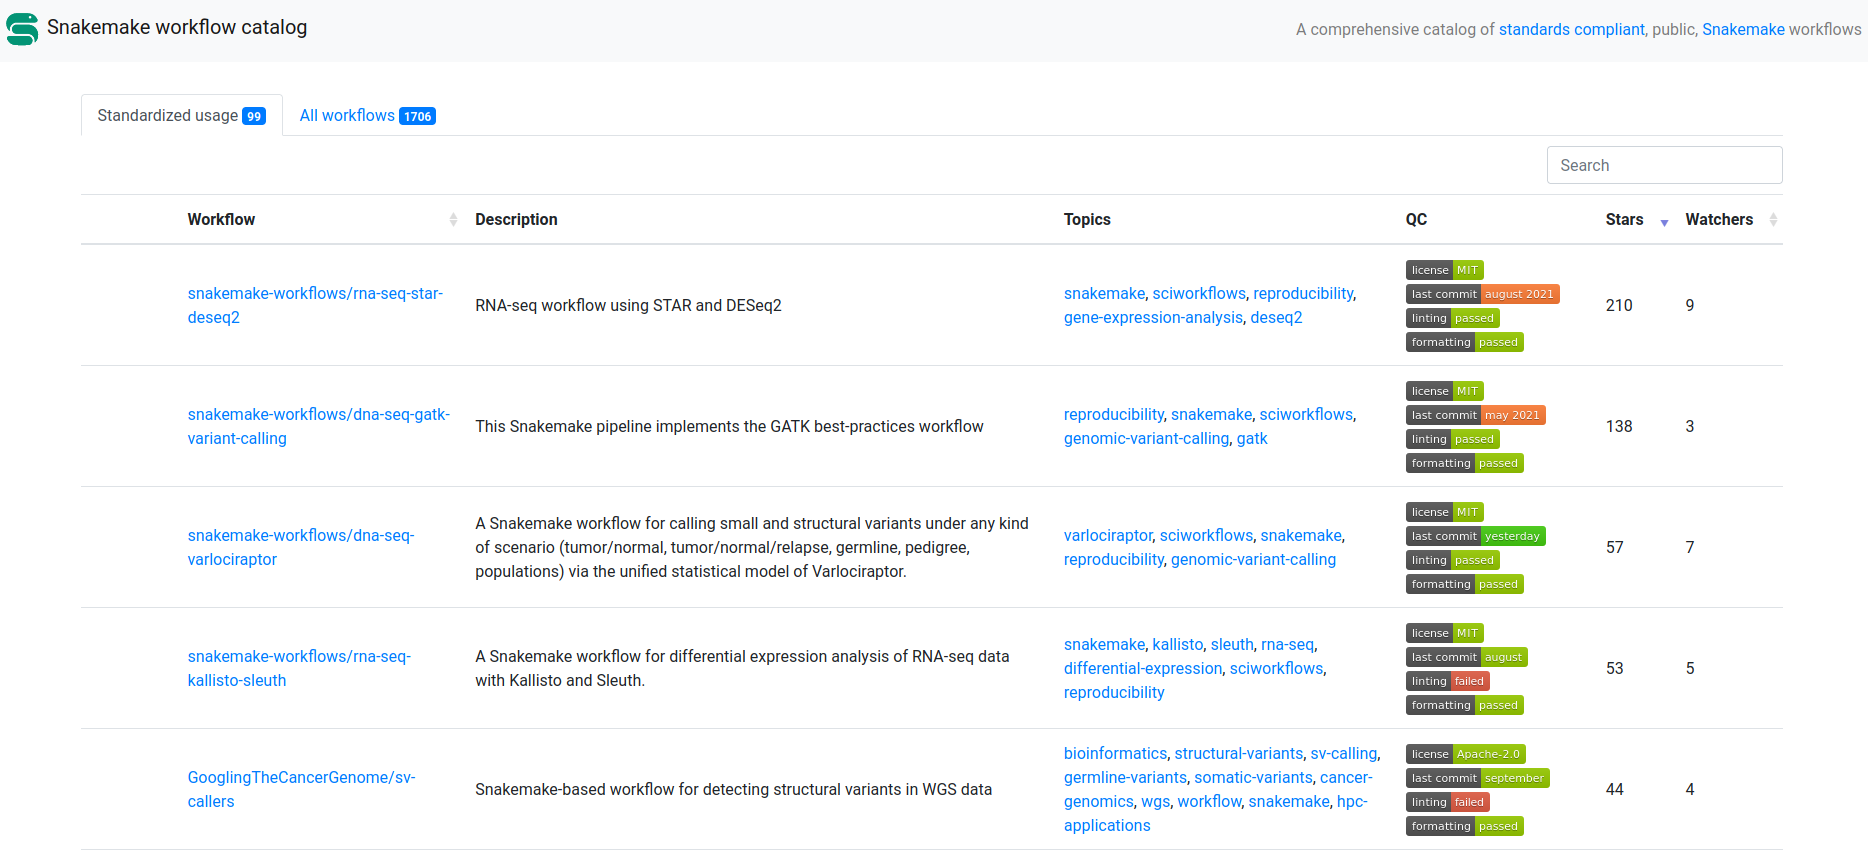
\includegraphics[width=\textwidth]{Snakemake/Snakemake_Workflow_Catalog.png}
				\vspace{0.5em}
				\caption*{Screenshot of the Workflow Catalogue}
			\end{figure}
		\end{column}
	\end{columns}
\end{frame}

%%%%%%%%%%%%%%%%%%%%%%%%%%%%%%%%%%%%%%%%%%%%%%%%%%%%%%%%%%%%%%%%%%%%%%%%%%%%%%%%
\subsection{Background}

%%%%%%%%%%%%%%%%%%%%%%%%%%%%%%%%%%%%%%%%%%%%%%%%%%%%%%%%%%%%%%%%%%%%%%%%%%%%%%%%
\begin{frame}[fragile]
	\frametitle{How does \Snakemake on a Cluster work?}
	\begin{columns}[T]
		\begin{column}{.5\textwidth}
			\only<3->{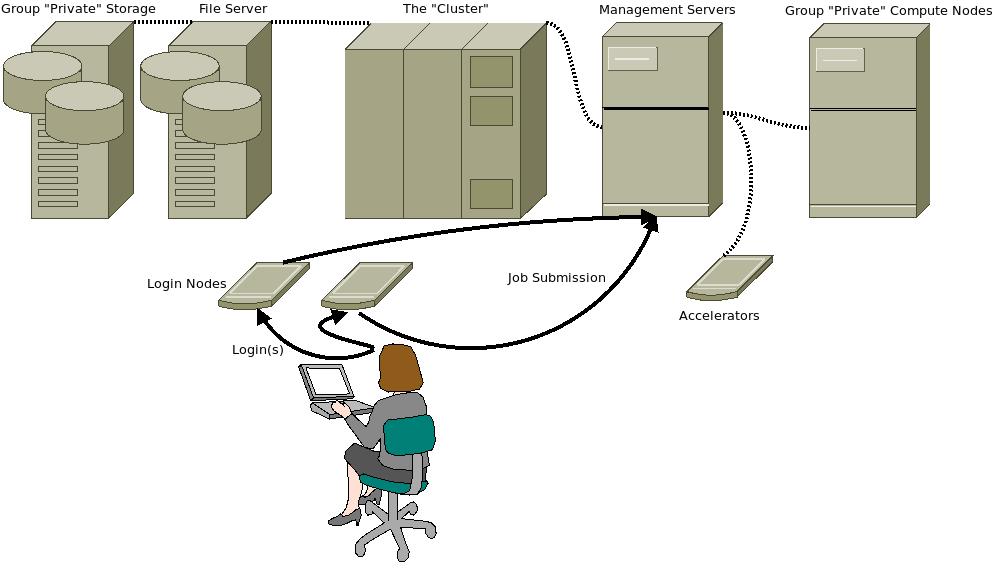
\includegraphics[width=0.95\textwidth]{misc/cluster_scheme.png}}
		\end{column}
		\begin{column}{.5\textwidth}
			\begin{itemize}[<+->]
				\item Snakemake is triggered on the command line:
				\begin{lstlisting}[language=Bash, style=Shell]
$ snakemake [<arguments>]
				\end{lstlisting} 
			    \item users need to fill in the parameters of their workflow (e.\,g. input path(s) in a file)
			    \item Snakemake will run on the login-node and spawn your jobs on the cluster using a
			    \item cluster specific configuration file 
			\end{itemize}
		    \pause
			It is capable to remove temporary files and support various archiving systems.
		\end{column}
	\end{columns}
\end{frame}

%%%%%%%%%%%%%%%%%%%%%%%%%%%%%%%%%%%%%%%%%%%%%%%%%%%%%%%%%%%%%%%%%%%%%%%%%%%%%%%%
\begin{frame}<handout:0>
  \frametitle{"Spawn Jobs on a Cluster?!" - What does it mean?}
  \begin{hint}
  	Here, we explain to users the difference between PC and Servers and HPC Systems. You will get the Admin background, only.
  \end{hint}
  \pause
  \begin{itemize}[<+->]
  	\item \Snakemake is triggered on a login-node, only.
  	\item It will submit jobs \ldots
  	\item \ldots and keeps running (without CPU load!) to monitor the job execution.
  	\item depending on the workflow, it will download or plot with minor CPU load on the login node. (Hard to notice with a simple \verb*|top| command.)
  \end{itemize}
\end{frame}

%%%%%%%%%%%%%%%%%%%%%%%%%%%%%%%%%%%%%%%%%%%%%%%%%%%%%%%%%%%%%%%%%%%%%%%%%%%%%%%%
\begin{frame}
   \frametitle{Benefit of Cluster Usage}
   \begin{columns}
   	 \begin{column}{0.6\textwidth}
   	 	\centering
   	 	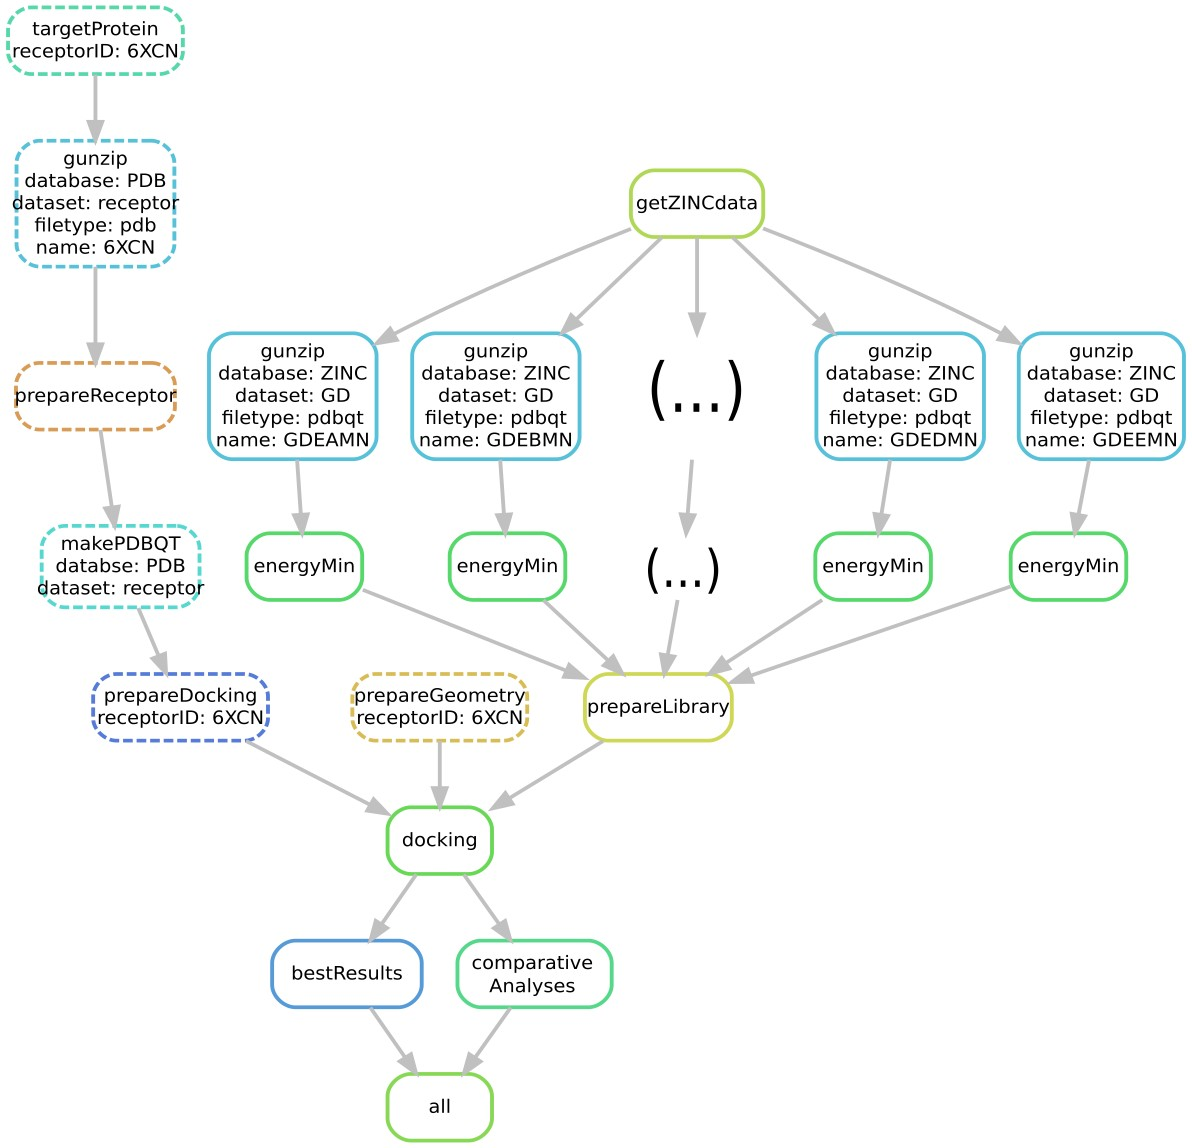
\includegraphics[width=0.8\textwidth]{workflows/molecular_screening_dag.jpeg}
   	 \end{column}
     \begin{column}{0.6\textwidth}
     	{\footnotesize
     		\Snakemake offers
     		\begin{itemize}[<+->]
     		  \item to carry out Nextflow wrappers
     		  \item to react on your input \newline $\Rightarrow$  more samples, more jobs
     		  \item to be a remedy to I/O contention
     		  \item to be ready for real time \newline computation with cluster support
     		  \item to support you from your input \newline to publication
     		  \item \ldots
     		\end{itemize}
     	}
     \end{column}
   \end{columns}
\end{frame}
	